\documentclass[11pt]{article}
\usepackage{algorithm2e}
\usepackage[italian]{babel}
\usepackage[document]{ragged2e}
\justifying
\usepackage{amsfonts, amssymb, amsmath}
\usepackage{cancel}
\usepackage{float}
\usepackage{mathtools}
\usepackage[margin=3cm]{geometry}
% \setcounter{secnumdepth}{0}
\usepackage{hyperref}
\hypersetup{
    colorlinks,
    citecolor=black,
    filecolor=black,
    linkcolor=black,
    urlcolor=black
}

\tolerance=1
\emergencystretch=\maxdimen
\hyphenpenalty=10000
\hbadness=10000

\begin{document}
\begin{titlepage}
    \begin{center}
        \vspace*{1.5cm}
            
        \Huge
        \textbf{Tweet Analysis}
            
        \vspace{0.3cm}
        \LARGE
        Relazione finale\\[0.2em]

        \vspace{1.5cm}
          
        \begin{minipage}[t]{0.47\textwidth}
            \begin{center}
                \parbox{50mm}{\centering\large {\bf Cheikh Ibrahim $\cdot$ Zaid} \\[0.2em] PO Operativo \\[0.3em] Matricola: \texttt{0000974909}}\\[2em]
                \parbox{50mm}{\centering\large {\bf Lee $\cdot$ Qun Hao Henry} \\[0.2em] Developer \\[0.3em] Matricola: \texttt{0000990259}}
            \end{center}
		\end{minipage}
		\hfill
		\begin{minipage}[t]{0.47\textwidth}\raggedleft
            \begin{center}
                \parbox{50mm}{\centering\large {\bf Xia $\cdot$ Tian Cheng} \\[0.2em] Scrum master \\[0.3em] Matricola: \texttt{0000975129}}\\[2em]
                \parbox{50mm}{\centering\large {\bf Paris $\cdot$ Manuel} \\[0.2em] Developer \\[0.3em] Matricola: \texttt{0000997526}}
            \end{center}
		\end{minipage}  
            
        \vspace{6cm}
            
        Anno accademico\\
        $2022 - 2023$
            
        \vspace{0.8cm}
            
            
        \Large
        Corso di Ingegneria del Software\\
        Alma Mater Studiorum $\cdot$ Università di Bologna\\
            
    \end{center}
\end{titlepage}
\pagebreak


\tableofcontents
\newpage


\section{Descrizione del prodotto}

\subsection{Scope}

\subsection{Casi d'uso}

\subsection{Diagramma delle classi}

%%%

\newpage
\section{Descrizione degli sprint}

\subsection{Sprint 1}
\subsubsection{Sprint goal}

\subsubsection{Backlog}

\subsubsection{Burndown}
\begin{figure}[H]
    \centering
    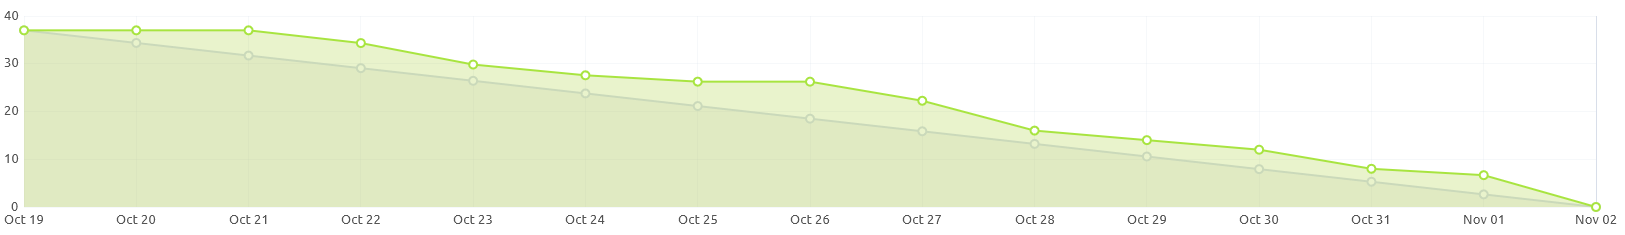
\includegraphics[width=12cm]{./img/sprint1/burndown.png}
    \caption{Burndown}
\end{figure}
\begin{figure}[H]
    \centering
    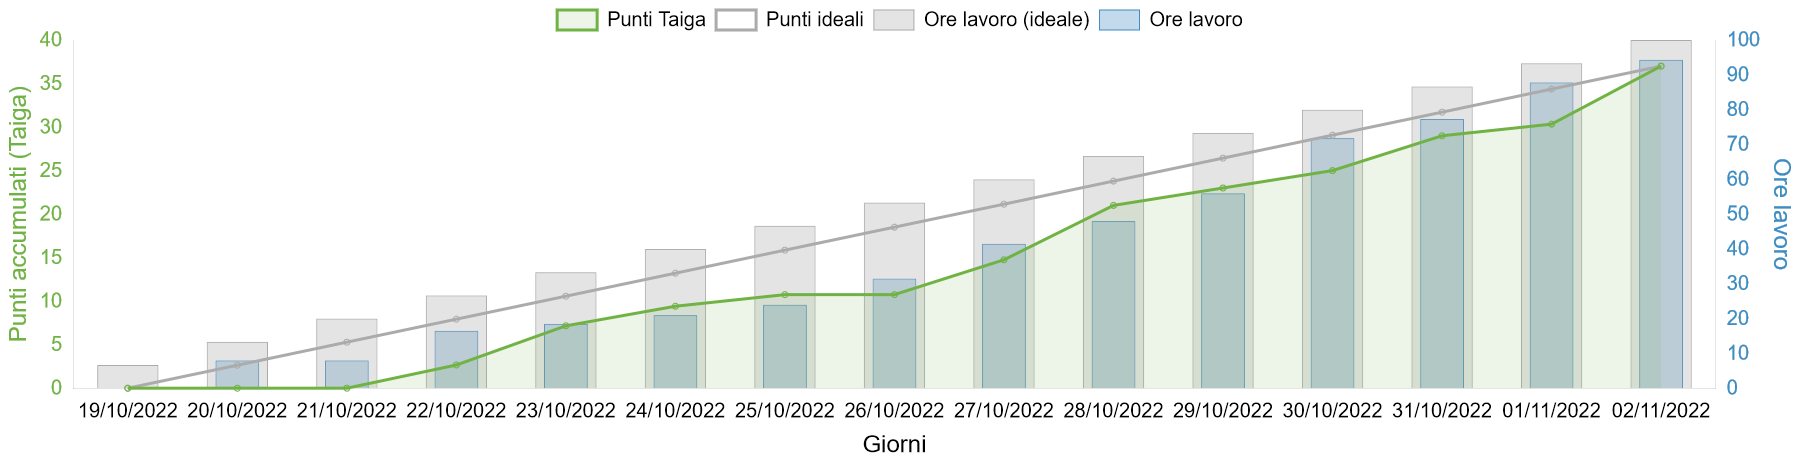
\includegraphics[width=12cm]{./img/sprint1/worktime.png}
    \caption{Progresso dei punti (asse a sinistra) e ore di lavoro (asse a destra)}
\end{figure}

\subsubsection{Retrospettiva}


\subsection{Sprint 2}
\subsubsection{Sprint goal}

\subsubsection{Backlog}

\subsubsection{Burndown}
\begin{figure}[H]
    \centering
    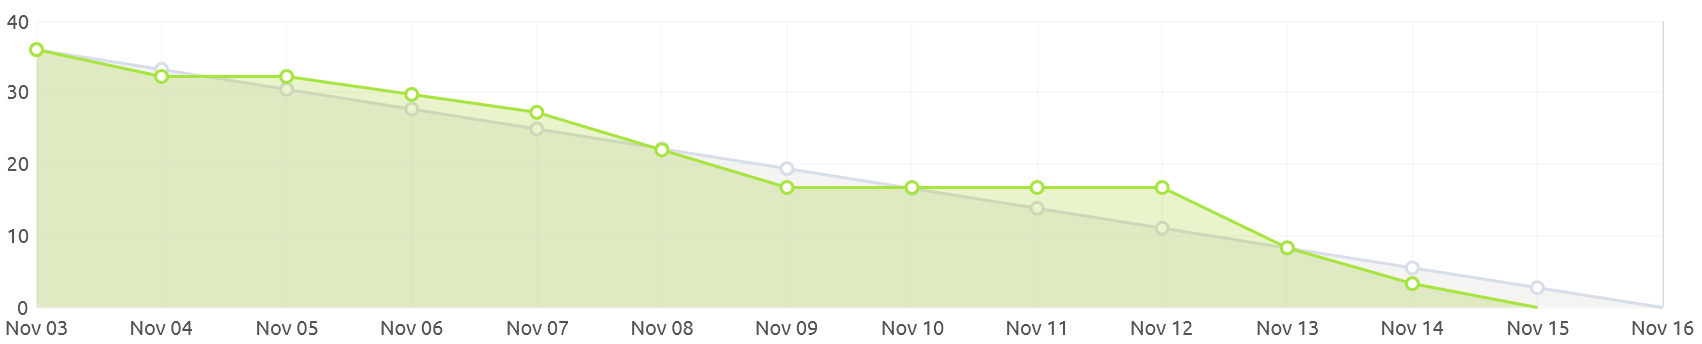
\includegraphics[width=12cm]{./img/sprint2/burndown.png}
    \caption{Burndown}
\end{figure}
\begin{figure}[H]
    \centering
    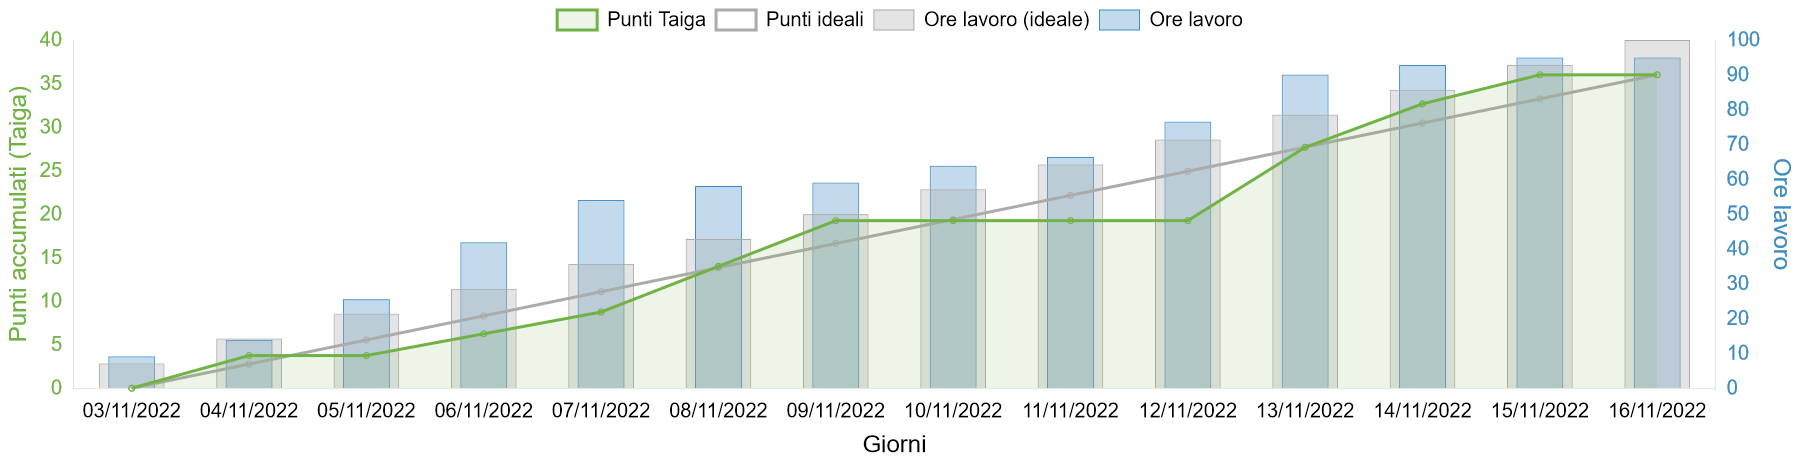
\includegraphics[width=12cm]{./img/sprint2/worktime.png}
    \caption{Progresso dei punti (asse a sinistra) e ore di lavoro (asse a destra)}
\end{figure}

\subsubsection{Retrospettiva}


\subsection{Sprint 3}
\subsubsection{Sprint goal}

\subsubsection{Backlog}

\subsubsection{Burndown}
\begin{figure}[H]
    \centering
    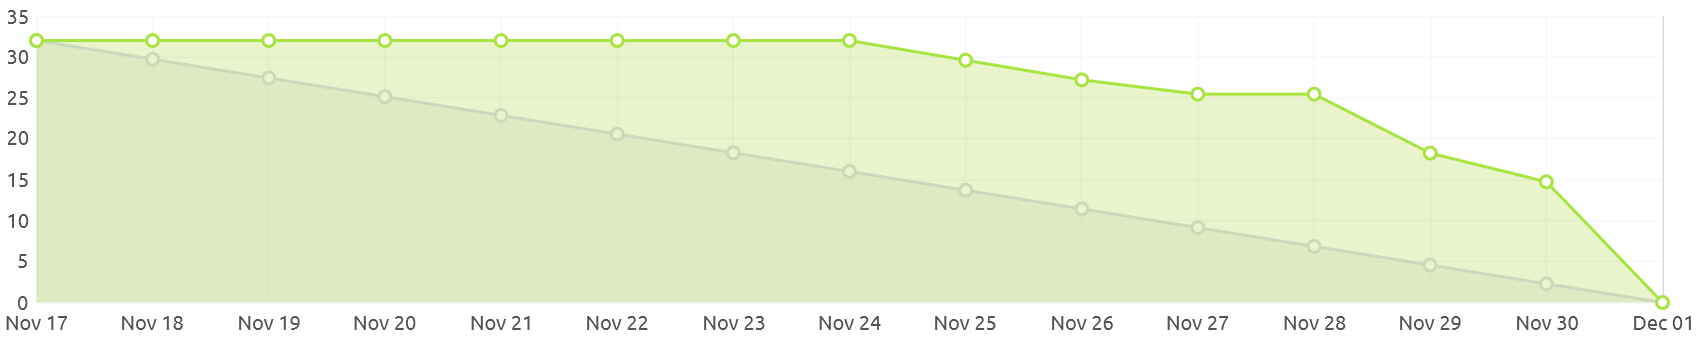
\includegraphics[width=12cm]{./img/sprint3/burndown.png}
    \caption{Burndown}
\end{figure}
\begin{figure}[H]
    \centering
    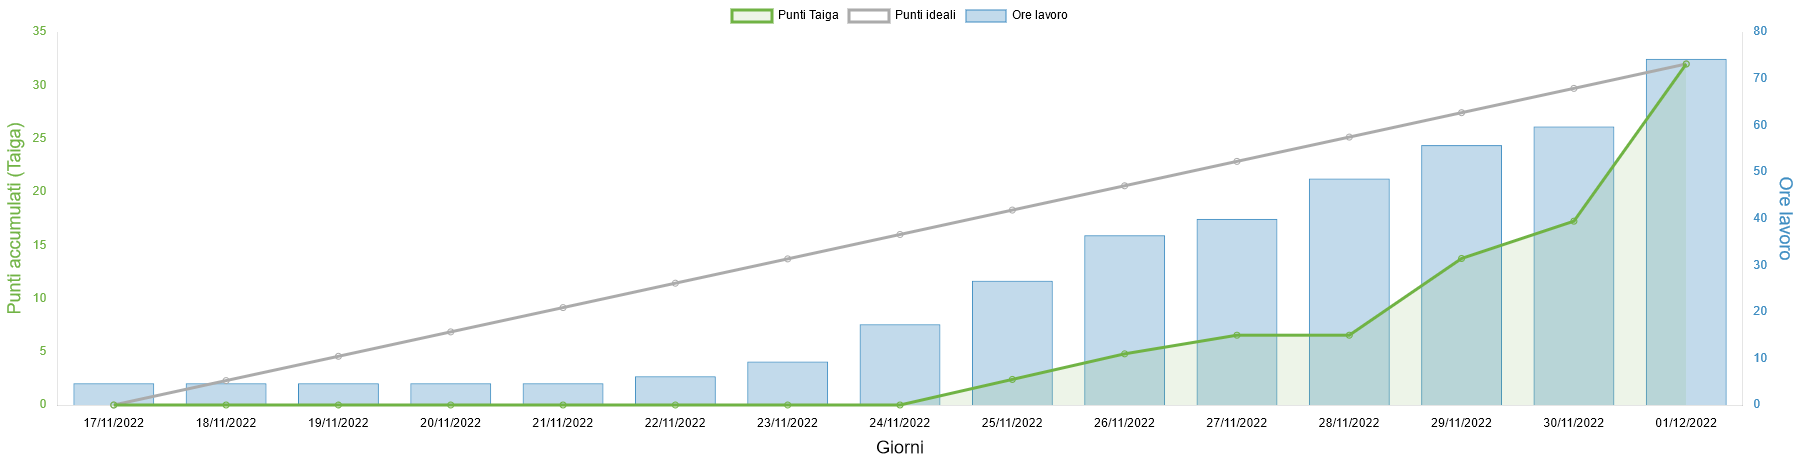
\includegraphics[width=12cm]{./img/sprint3/worktime.png}
    \caption{Progresso dei punti (asse a sinistra) e ore di lavoro (asse a destra)}
\end{figure}

\subsubsection{Retrospettiva}


\subsection{Sprint 4}
\subsubsection{Sprint goal}
\subsubsection{Backlog}
\subsubsection{Burndown}
\subsubsection{Retrospettiva}

%%%

\newpage
\section{Descrizione del processo}

\subsection{Team building}
\subsubsection{Scrumble}
\subsubsection{Escape the Boom}

\subsection{Gitinspector}

\subsection{Retrospettiva finale}

\subsection{Deployment}


\newpage
\section{Artefatti}

\end{document}

